\documentclass[french,12pt]{article}
\usepackage{babel}
\usepackage[utf8]{inputenc}%encodage des caractères
\usepackage[T1]{fontenc}%encodage de la police
\usepackage{graphicx}
\usepackage{amsmath}
\usepackage{hyperref}

\title{Rapport Conception Logiciel}
\author{Mathieu Goudal, Hugo Bosvy, Valère Sarfati, \\Edwin Bertin-Cohonner}
\date{25 Avril 2022}

\begin{document}

\maketitle

\begin{figure}[h]
	\begin{center}
		
\includegraphics[scale=0.5]{img/cartes.png}	
	\end{center}
\end{figure}

\begin{figure}`
	\begin{center}
		
\includegraphics[scale=0.7]{img/unicaen.png}	
	\end{center}
\end{figure}

\thispagestyle{empty}
\setcounter{page}{0}
\newpage

\tableofcontents
\newpage

\section{Introduction}

\subsection{Description du projet}

Nous avions pour but de coder en Python, un jeu qui s'intitule "Le président". Ce genre de jeu est un jeu de cartes où chaque joueur doit se débarrasser le plus rapidement possible de la totalité de ses cartes. Les joueurs ayant été les plus rapides à se débarrasser de leurs cartes ont droit à un avantage pour la partie suivante et inversement les plus lents se verront pénalisés par un handicap.\\
Le "2" est la carte la plus haute, tandis que le "3" est la plus basse. \\
Les cartes posées doivent toujours être supérieures à celles déjà jouées.\\
Lors d’une série, le jeu s’arrête lorsque plus aucun des participants ne peut ou ne veut jouer une carte supérieur. Ainsi, il n’est pas possible de faire une boucle comme par exemple As, 2 et repartir sur 3.


\subsection{Plan du rapport}

Nous évoquerons d'abord quels étaient nos objectifs de départ, puis nous détaillerons les différentes étapes de la création de notre projet avec les rôles de chacuns. Ensuite nous présenterons l'achitecture de ce projet et finalement nous présenterons certaines expérimentations et terminerons par une courte conclusion.

\section{Objectifs du projet}

Nous voulions développer une interface graphique pour jeux de cartes. Nous avons donc choisit le jeu de cartes "Président". Ce jeu peut se jouer à 4 joueurs sur la même machine. Nous avons décidé de proposer 4 thèmes différents: \textit{Basique}, \textit{Shingeki no Kyojin}, \textit{Harry Potter} et \textit{Avengers}.

\section{Fonctionnalités implémentées}

\subsection{Description des fonctionnalités}

Les possibilités du jeu sont multiples. A partir de l'accueil, il est possible de choisir le thème du plateau de jeu à partir de différents boutons; les boutons \texttt{Theme$\_$basique}, \texttt{Theme$\_$snk}, \texttt{Theme$\_$harrypotter}, et \texttt{Theme$\_$avengers}. Après avoir choisit son thème, il suffit d'appuyer sur le bouton "\texttt{Play}" pour lancer la partie.
\\\\
Une fois la partie lancée, un bouton "\texttt{Paramètre}" se trouve en haut à droite de l'écran, ce bouton ouvre une nouvelle fenêtre qui permet de changer de thème en cours de jeu, ou d'accéder aux règles du jeu.\\
Dans cette fenêtre se trouve aussi un bouton "\texttt{Exit}" permettant de retourner au plateau de jeu.
\\\\
En haut à gauche de l'écran se trouve un autre bouton "\texttt{Son}" permettant de couper et remettre la musique de fond.
\\\\
Un dernier bouton "\texttt{Jouer}", permet de jouer ses cartes selectionnées, ou de passer son tour.

\subsection{Organisation du projet}

Pour commencer, Valère et Edwin ont effectués plusieurs recherches sur la manière de coder en pygame. \\
Mathieu et Hugo, quant à eux, ont commencés à coder "\textsf{class$\_$carte}" qui leur a servit à définir les propriétés des cartes (sa valeur, son nom et sa couleur). Elle leur a aussi permit d'attribuer une image à chaque carte et sa "\textit{hitbox}" (surface cliquable de la carte).\\
Cette classe contient plusieurs fonctions:\\
\begin{itemize}
\item La fonction "\texttt{update()}" permet de définir la taille d'une carte.
\item La fonction "\texttt{maj$\_$image()}" permet d'attribuer le recto correspondant à sa carte.
\item La fonction "\texttt{$\_$str$\_$()}" permet de récupérer le nom exact de la carte dans la variable "\texttt{image$\_$recto} de la forme nom + couleurs.\\
\end{itemize}

Pour créer le paquet de carte, Mathieu et Hugo ont définit "\textsf{class$\_$deck}". Ils ont définit une variable "\texttt{type}" qui leur permettra par la suite de créer un jeu de 52 cartes ou un jeu vide grâce au fichier "\textsf{config}".\\
Cette classe contient plusieurs fonctions permettant de manipuler le paquet de cartes:\\
\begin{itemize}
\item La fonction "\texttt{mélanger()}" appel la fonction "\texttt{shuffle}" de la classe Python "\textsf{random}" afin de mélanger le jeu de cartes.
\item La fonction "\texttt{tirer()}" permet de tirer la dernière carte du jeu et de la supprimer du paquet.
\item La fonction "\texttt{ajouter()}" permet d'ajouter une carte à un paquet.
\item La fonction "\texttt{enlever()}" permet d'enlever une carte à d'un paquet.\\
\end{itemize}

Ensuite ils ont créés des joueurs dans "\textsf{class$\_$joueur}". Ces joueurs possèdent un "\texttt{id}" et une "\texttt{main}" créée à partir de "\textsf{class$\_$deck}".
\\\\
Pour le fonctionnement du jeu, toutes les fonctions ont été codées dans \textsf{president}" par Mathieu et Hugo. \\
Dans cette classe a été créée la \texttt{pioche} (à partir de "\texttt{class$\_$deck}"). Cette pioche est un jeu de 52 cartes mélangées qui nous sert à construire les mains des joueurs.\\
La \texttt{défausse}, quant à elle, est un deck vide également codé à partir de "\texttt{class$\_$deck}".\\
\texttt{dernier$\_$joueur} est le dernier joueur à avoir joué une ou plusieurs carte(s).\\
\texttt{nb$\_$carte$\_$tour} est le nombre de cartes jouées par le joueur qui a ouvert le tour, c'est-à-dire, le nombre de cartes à jouer tout le long du tour.\\
\texttt{joueur$\_$en$\_$cours} sert à savoir qui est le joueur qui est en train de jouer.\\
Nos 4 joueurs et leurs mains ont été créés ici grâce à de multiples fonctions:\\

\begin{itemize}
\item "\texttt{dessine$\_$main$\_$joueur()}" parcourt la main d'un joueur et dessine chaque carte de la main à l'écran. Les mains sont dessinées différemments en fonction de l'id du joueur c'est-à-dire de son placement sur l'écran (haut, bas, droite ou gauche). Cette fonction permet également de monter les cartes lorsqu'elles sont sélectionnées (elles se déplacent encore différemments selon l'id du joueur).\\

\item "\texttt{display$\_$main$\_$joueur()}" fait appel à la fonction "\texttt{dessine$\_$main$\_$joueur()}" et permet de dessiner toutes les mains de tous les joueurs en même temps. Grâce aux paramètre \texttt{x} et \texttt{y} de la fonction "\texttt{dessine$\_$main$\_$joueur()} l'affichage des cartes est dynamique, cela veut dire que selon la taille de la main du joueur, les cartes seront toujours centrées. En effet, le x ou le y changera automatiquement, en fonction de l'id du joueur, quand le joueur jouera une carte. Nous avons attribué une formule au \texttt{x} et au \texttt{y} qui est : (longeur ou largeur (selon l'id) de l'écran/2)-((longeur ou largeur (selon l'id) d'une carte + la longeur de la main du joueur*30)/2).Lorsque le joueur va jouer une carte, sa main va se centrer grâce à cette formule.\\

\item "\texttt{display$\_$dessine$\_$defausse()}" permet de dessiner la défausse, c'est-à-dire, l'endroit où les cartes jouées sont placées. Cette défausse est parcourue et chaque carte qu'elle contient est dessinée et placée au centre du plateau.\\

\item "\texttt{joueur$\_$suivant()}" permet de changer de joueur.\\

\item "\texttt{carte$\_$select()}" permet au joueur en cours de sélectionner les cartes qu'il veut jouer. Cette fonction fait en sorte que le joueur puisse seulemnt sélectionner des cartes de mêmes valeurs.
En effet, si le joueur sélectionne des cartes de valeurs différentes, alors les premières cartes sélectionnées seront automatiquement déselectionner.\\

\item "\texttt{jouer$\_$carte()}" permet de placer les cartes selectionnées dans la défausse, si elle respecte les conditions fixées:
\begin{enumerate}
\item Le premier joueur à ouvrir le tour, détermine le nombre de cartes qu'il faudra jouer tout le reste du tour grâce à \texttt{nb$\_$carte$\_$tour}.
\item Si le nombre de cartes n'est pas respecté, un message s'affiche et le joueur a la possibilité de ré-essayer de jouer. 
\item Si un joueur joue la carte "2", le tour se ferme automatiquement et c'est encore à lui de ré-ourvir le nouveau tour.  
\item Si les 4 dernières cartes posées dans la défausse sont de mêmes hauteurs, le tour se ferme; c'est la règle du \textit{carré magique}.
\item Si 3 joueurs passent leur tour, le tour se ferme et la main revient à \texttt{dernier$\_$joueur}. \\
\end{enumerate}

\item "\texttt{fermer$\_$tour()}" permet de vider la défausse.\\

\item "\texttt{fin$\_$game()}" nous informe de la fin de la partie, pour pouvoir lancer la fenêtre de fin de jeu.\\

\item "\texttt{main$\_$vide()}" permet de passer automatiquement le tour d'un joueur n'ayant plus de cartes.
 
\end{itemize}

Mathieu a choisit de ranger les différents éléments graphiques dans différentes classes. Il y a donc une classe "\texttt{bouton}", "\texttt{couleur}", "\texttt{texte}", "\texttt{image}", "\texttt{bruitage}".
\\\\
Enfin, Valère et Edwin se sont occupés du rapport, tandis que Mathieu de l'interface graphique.

\section{Architecture du projet}

Diagramme de toutes les classes (et leurs dépendances):

\begin{center}
	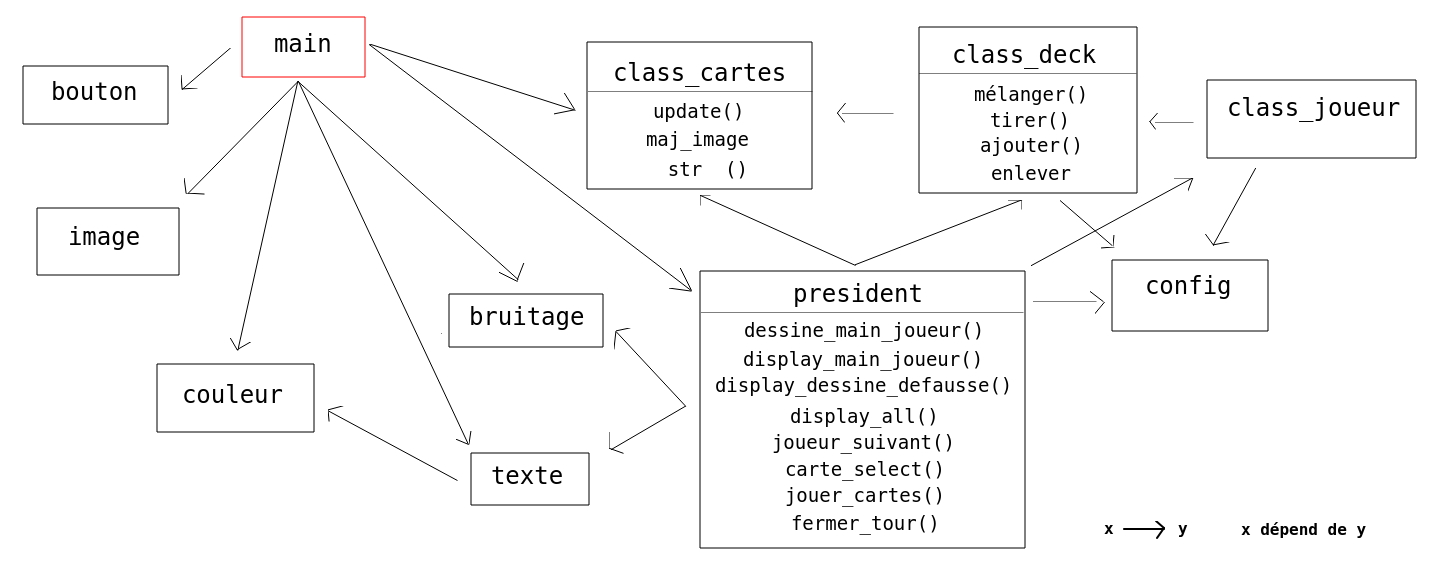
\includegraphics[scale=0.3]{img/diagramme_classes.png}	
\end{center}


\section{Expérimentations}

Lorsque vous lancez le jeu, vous arrivez sur une fenêtre d'accueil avec 5 boutons, le bouton \textbf{Play} et les boutons des 4 thèmes:

\begin{center}
	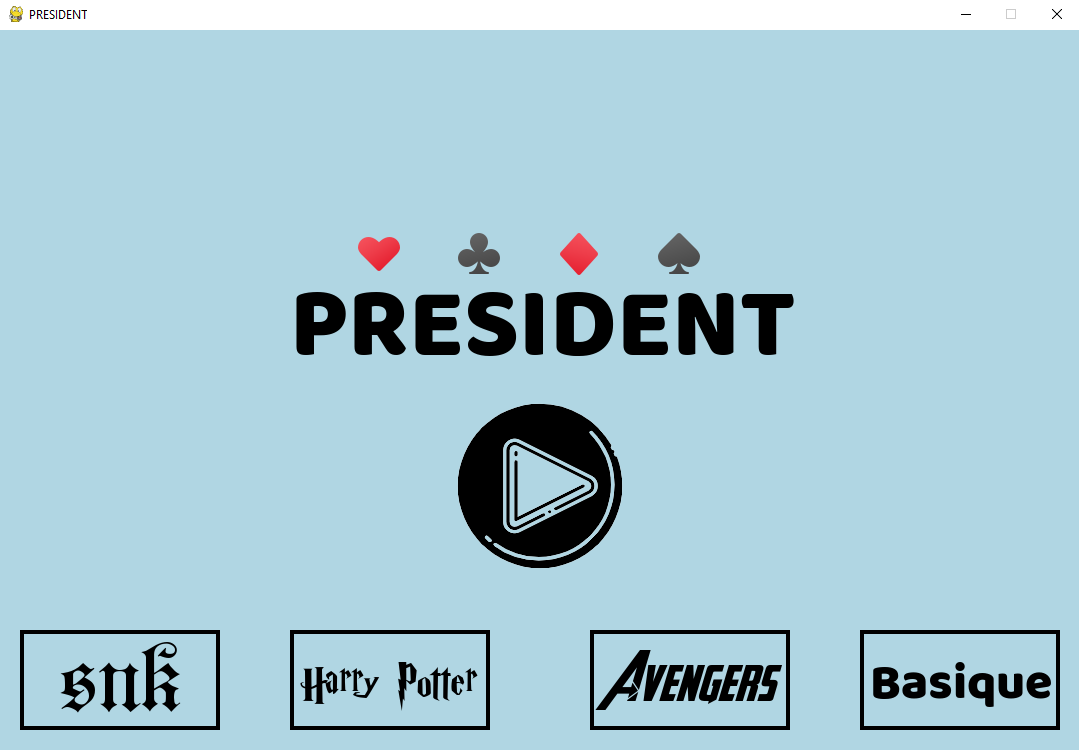
\includegraphics[scale=0.4]{img/accueil.png}
\end{center}

Vous pouvez choisir de changer de thème. Le fond, la musique, et les cartes seront différents:

\begin{center}
	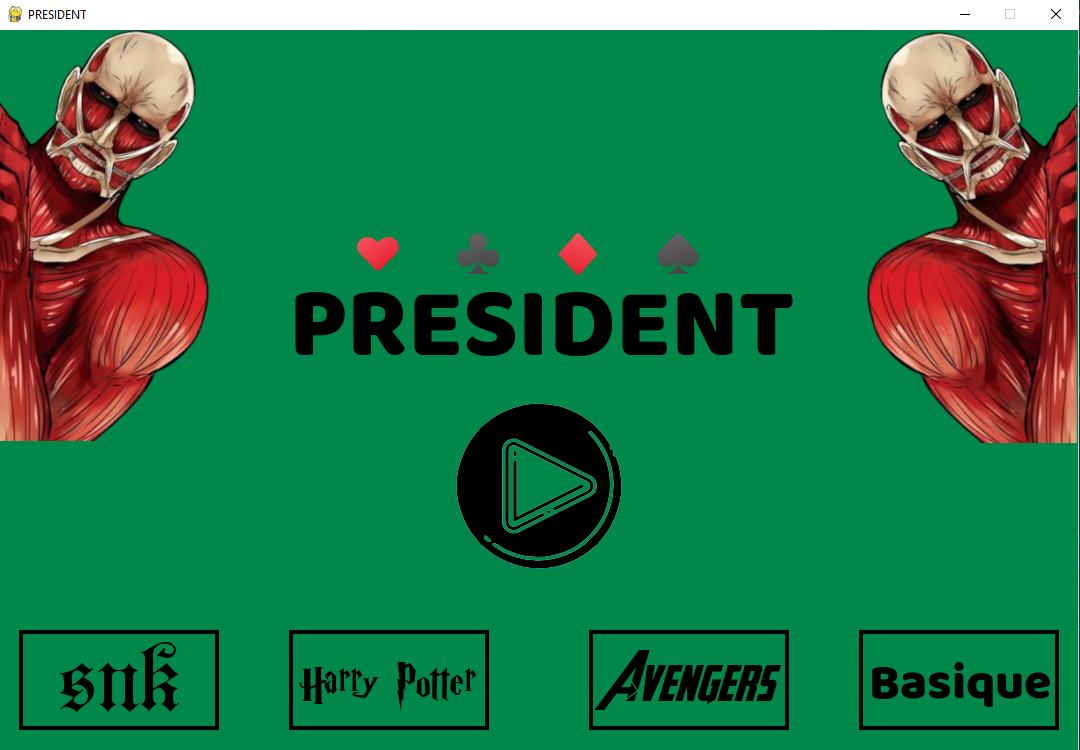
\includegraphics[scale=0.3]{img/accueil_snk.png}\\
	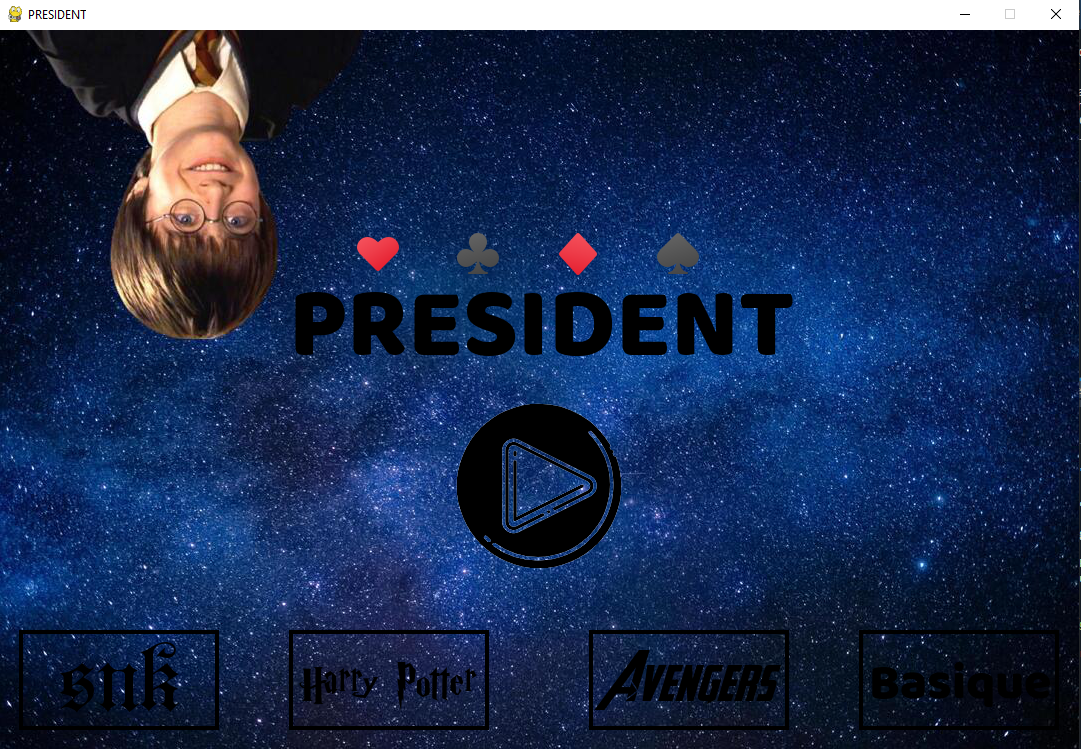
\includegraphics[scale=0.3]{img/accueil_hp.png}\\
	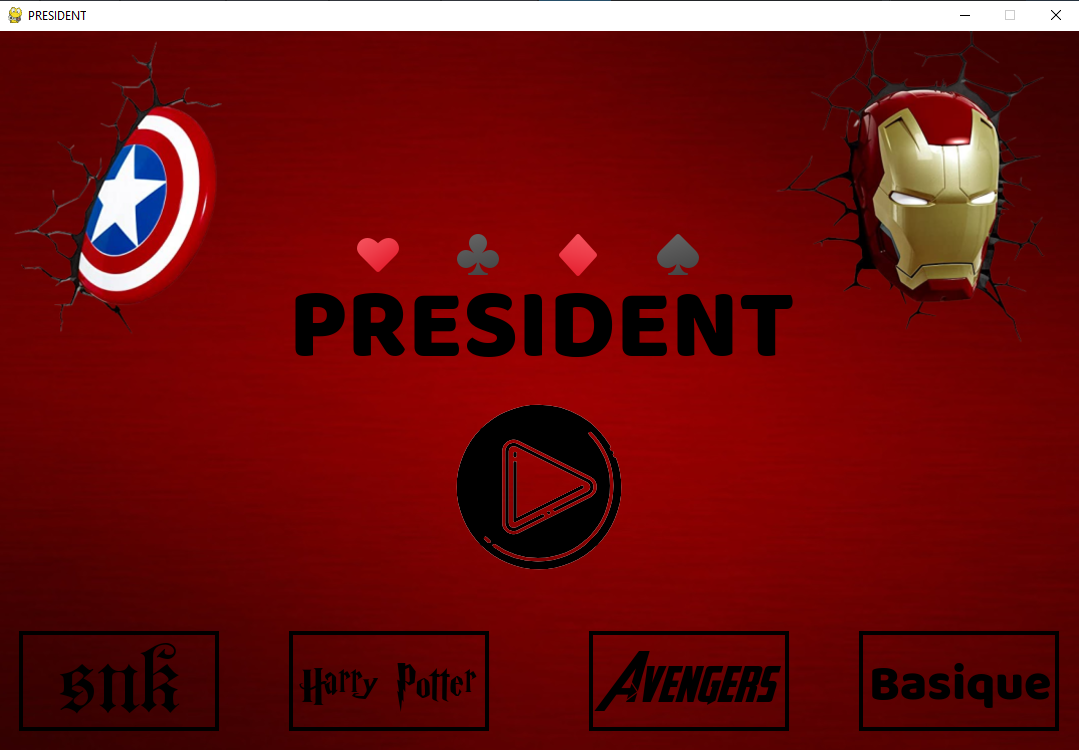
\includegraphics[scale=0.3]{img/accueil_avengers.png}
\end{center}

Après avoir choisit votre thème et cliqué sur le bouton \textbf{Play}, une page vous annoncera que le joueur 1 débute la partie. Cliquez n'importe où sur l'écran afin de passer au plateau de jeu:

\begin{center}
	
\includegraphics[scale=0.3]{img/joueur1.png}\\
	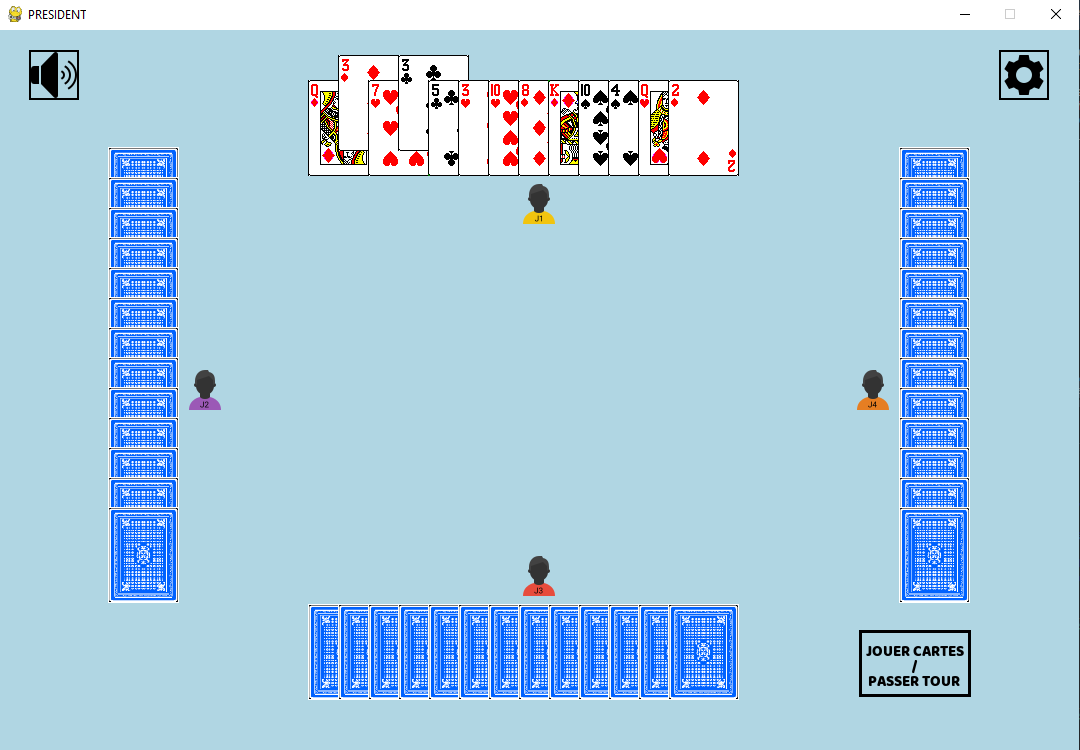
\includegraphics[scale=0.3]{img/jeu.png}
\end{center}

Le joueur 1 pourra alors sélectionner ses cartes (mais que les cartes de même hauteur afin de constituer des simples, des pairs, des brelans ou des carrés). Une fois ses cartes choisies, il suffira d'appuyer sur le bouton \textbf{Jouer cartes} pour les poser au centre du plateau. Une nouvelle fenêtre s'ouvrira afin d'informer les joueurs que c'est au tour du deuxième, pour qu'ils puissent se préparer à changer de joueurs.
La main affichée sera celle du joueur 2 et les cartes du joueur 1 seront posées au centre:

\begin{center}
	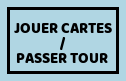
\includegraphics[scale=0.8]{img/jouer_cartes.png}\\
	
\includegraphics[scale=0.3]{img/joueur2.png}\\
	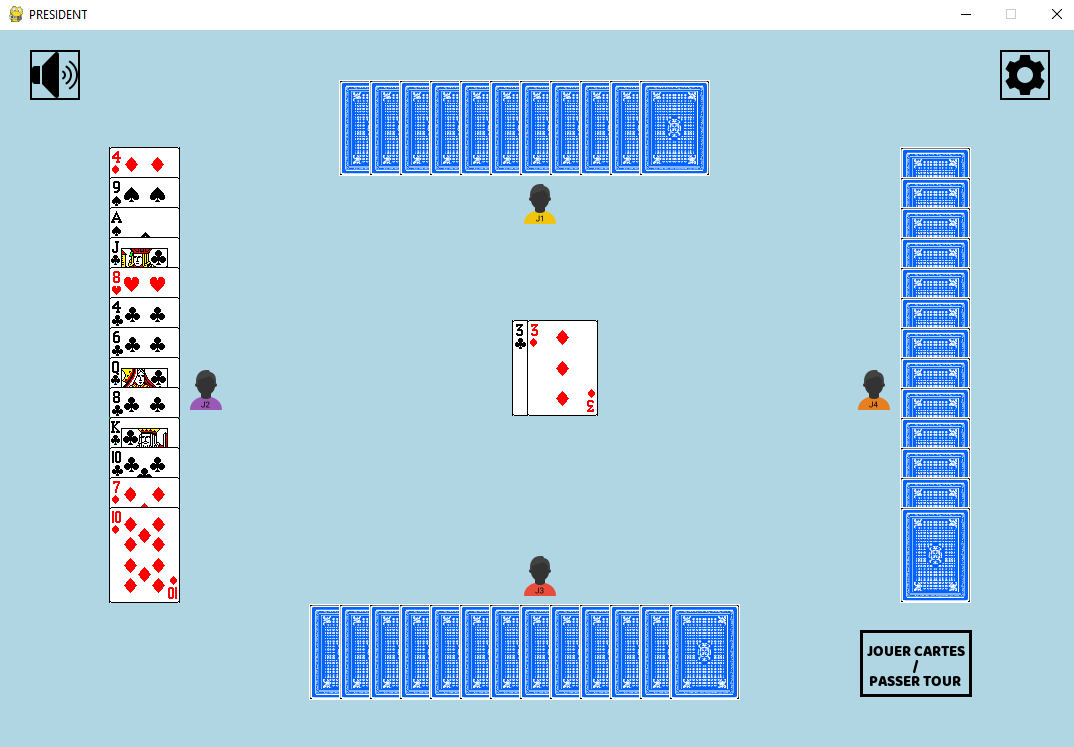
\includegraphics[scale=0.3]{img/cartes_posees.png}
\end{center}

Si un joueur ferme le tour en cours, une fenêtre l'en informera:

\begin{center}
	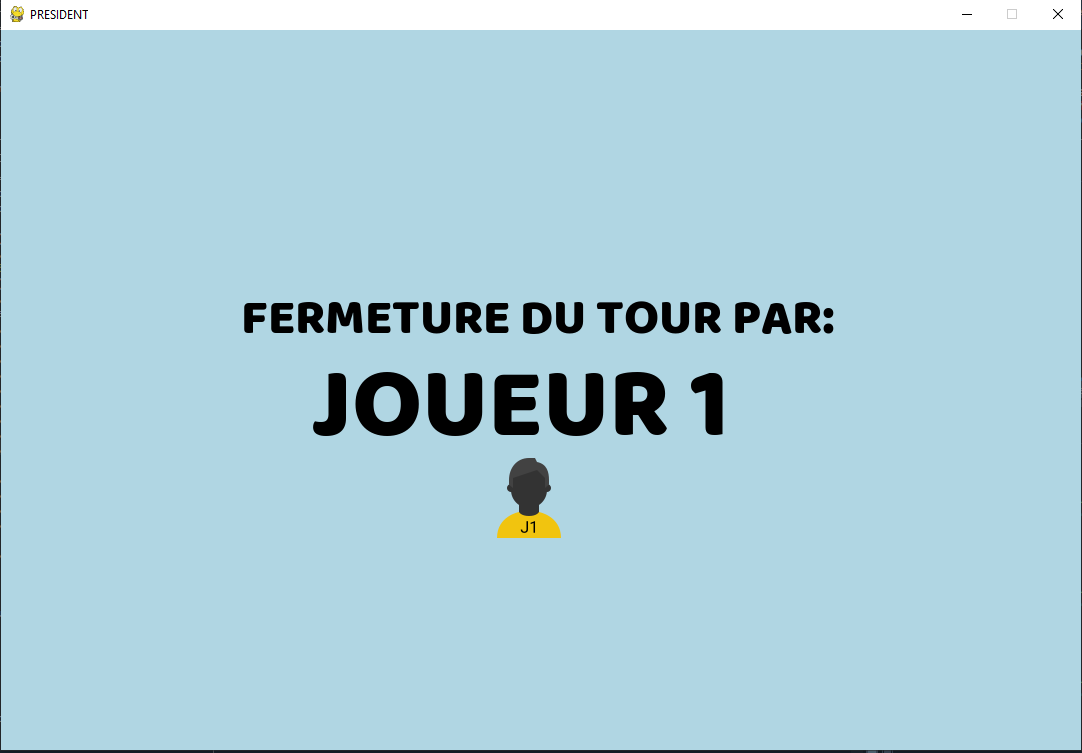
\includegraphics[scale=0.3]{img/fermeture.png}
\end{center}

Durant la partie, il sera possible de couper ou rallumer la musique à l'aide d'un bouton situé en haut à gauche. Selon sa forme, vous saurez si le son est coupé ou non:

\begin{center}
	
\includegraphics[scale=0.8]{img/son.png}
\end{center}

Il est également possible d'accéder aux paramètres avec un autre bouton situé en haut à droite. Une page s'ouvrira avec les règles du jeu et la possibilité de changer de thème en pleine partie. Cliquez sur la flèche en haut à droite afin de revenir à la partie:

\begin{center}
	
\includegraphics[scale=1.0]{img/parametres.png}\\
	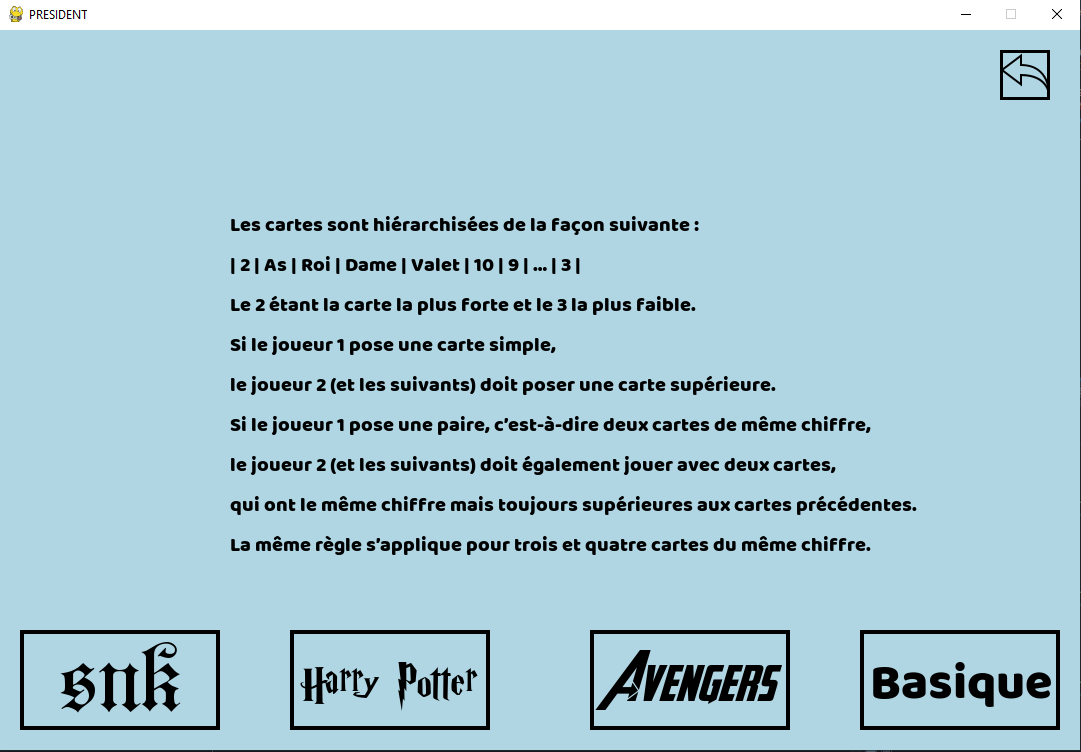
\includegraphics[scale=0.3]{img/regles.png}
\end{center}

Pendant la partie, si vous jouez des cartes qui ne sont pas possible (cartes trop basses ou nombres de cartes non respecté) une fenêtre vous informera que c'est impossible et vous aurez la possibilité de ré-essayer d'autres cartes ou de passer votre tour (avec le même bouton que pour jouer ses cartes):

\begin{center}
	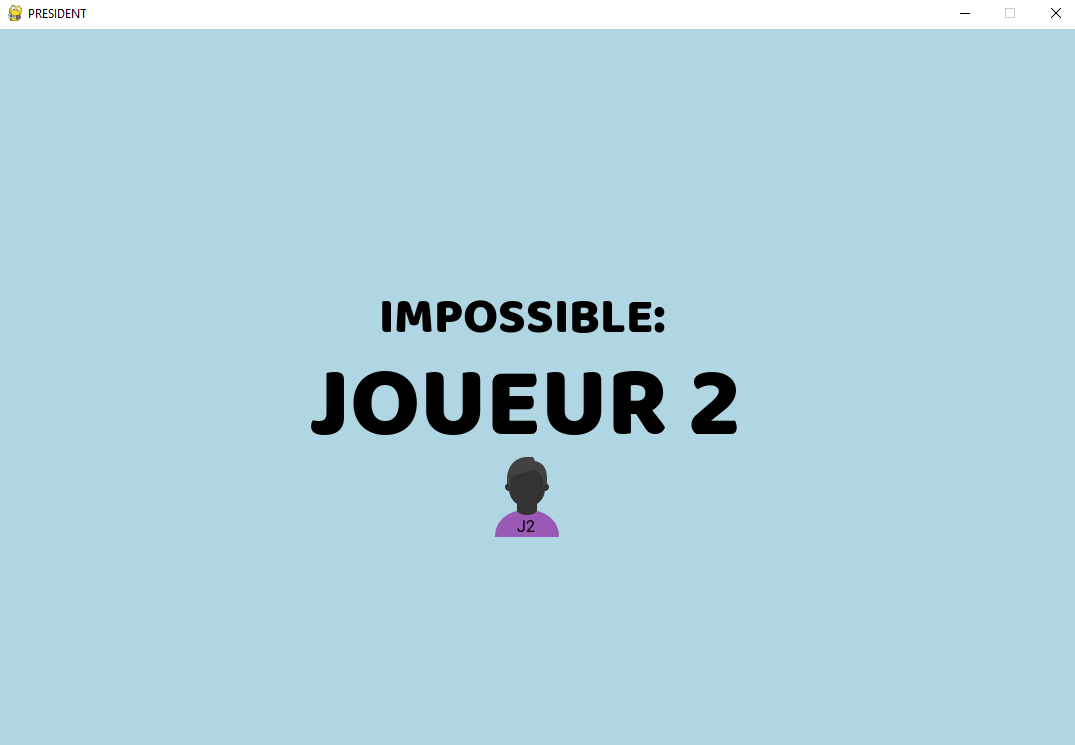
\includegraphics[scale=0.3]{img/impossible.png}
\end{center}

Lorsqu'il ne reste qu'un joueur en jeu, la partie se finit; une page s'ouvre avec un bouton pour fermer la fenêtre Pygame:

\begin{center}
	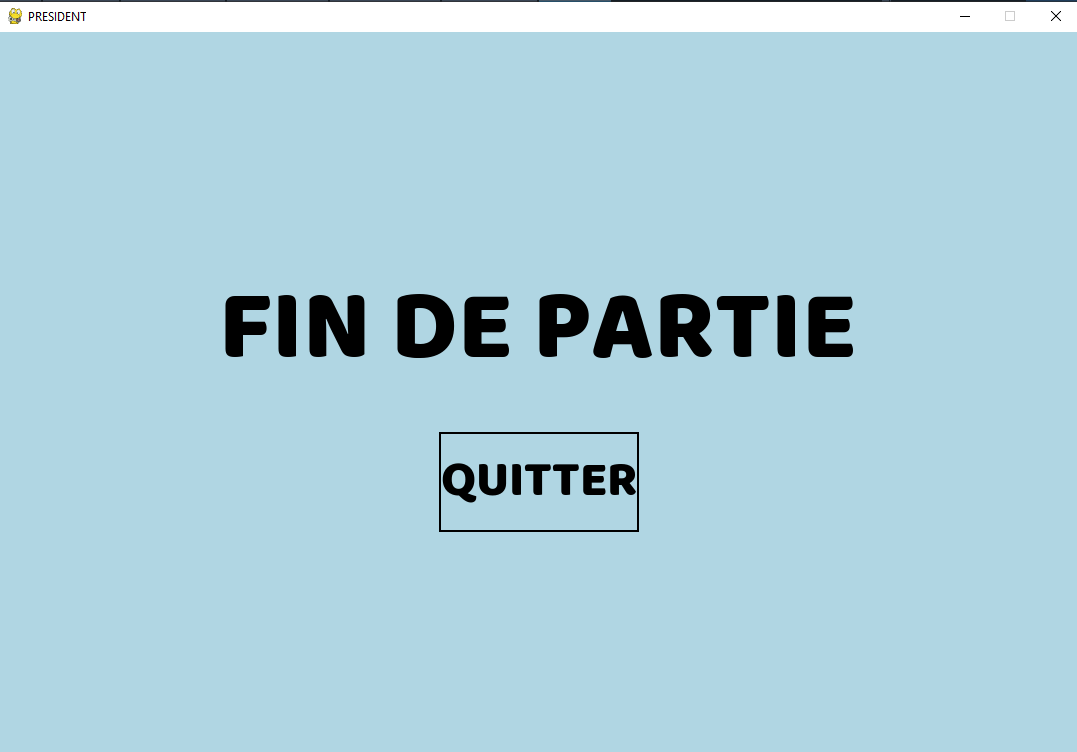
\includegraphics[scale=0.3]{img/fin_game.png}
\end{center}

\section{Conclusion}

Nous avons donc un jeu complet avec plusieurs fonctionnalités et choix de thèmes. Nous avons également réussit à implémenter presque toutes les règles telles que le "\textit{carré magique}", le joueur qui ferme le tour, ouvre le suivant, le "2" est la meilleure carte, l'obligation de poser le même nombre de cartes que le joueur précédent...etc\\
C'était bien l'objectif que nous nous étions fixés et nous en sommes fiers, mais pour améliorer notre jeu nous aurions pu faire un système de partie en boucle (c'est-à-dire, le président de la première partie devrait donner 2 de ses pires cartes au trou du cul à la seconde partie), ou encore la règle du "\textit{ta gueule}"

\end{document}